\RequirePackage{luatex85}
\documentclass[border=1pt]{standalone}

\usepackage{tikz}
\usepackage{fixltx2e}
\usetikzlibrary{math, arrows, patterns}

\def\hexagonsize{0.5cm}
\pgfdeclarepatternformonly
	{hexagons}% name
	{\pgfpointorigin}% lower left
	{\pgfpoint{3*\hexagonsize}{0.866025*2*\hexagonsize}}%  upper right
	{\pgfpoint{3*\hexagonsize}{0.866025*2*\hexagonsize}}%  tile size
	{% shape description
	  \pgfsetlinewidth{0.4pt}
	  \pgftransformshift{\pgfpoint{0mm}{0.866025*\hexagonsize}}
	  \pgfpathmoveto{\pgfpoint{0mm}{0mm}}
	  \pgfpathlineto{\pgfpoint{0.5*\hexagonsize}{0mm}}
	  \pgfpathlineto{\pgfpoint{\hexagonsize}{-0.866025*\hexagonsize}}
	  \pgfpathlineto{\pgfpoint{2*\hexagonsize}{-0.866025*\hexagonsize}}
	  \pgfpathlineto{\pgfpoint{2.5*\hexagonsize}{0mm}}
	  \pgfpathlineto{\pgfpoint{3*\hexagonsize+0.2mm}{0mm}}
	  \pgfpathmoveto{\pgfpoint{0.5*\hexagonsize}{0mm}}
	  \pgfpathlineto{\pgfpoint{\hexagonsize}{0.866025*\hexagonsize}}
	  \pgfpathlineto{\pgfpoint{2*\hexagonsize}{0.866025*\hexagonsize}}
	  \pgfpathlineto{\pgfpoint{2.5*\hexagonsize}{0mm}}
	  \pgfusepath{stroke}
	}

\tikzstyle{distArrow} = [<<->>, shorten >=8pt, shorten <=8pt, thick, line width=4pt]
\tikzstyle{dist2Arrow} = [|<->|, thick, line width=4pt]
\tikzstyle{pointer} = [->, shorten >=8pt, shorten <=14pt, thick, line width=2pt]
\tikzstyle{textStyle} = [fill=white!90!black, font=\Huge]
\tikzstyle{textLine} = [pos=0.5,sloped,above, font=\Huge, fill=white]
\tikzstyle{lineStyle} = [line width=4pt,dotted]
\tikzstyle{line2Style} = [black!50!white, line width=4pt,dashed]


\begin{document}
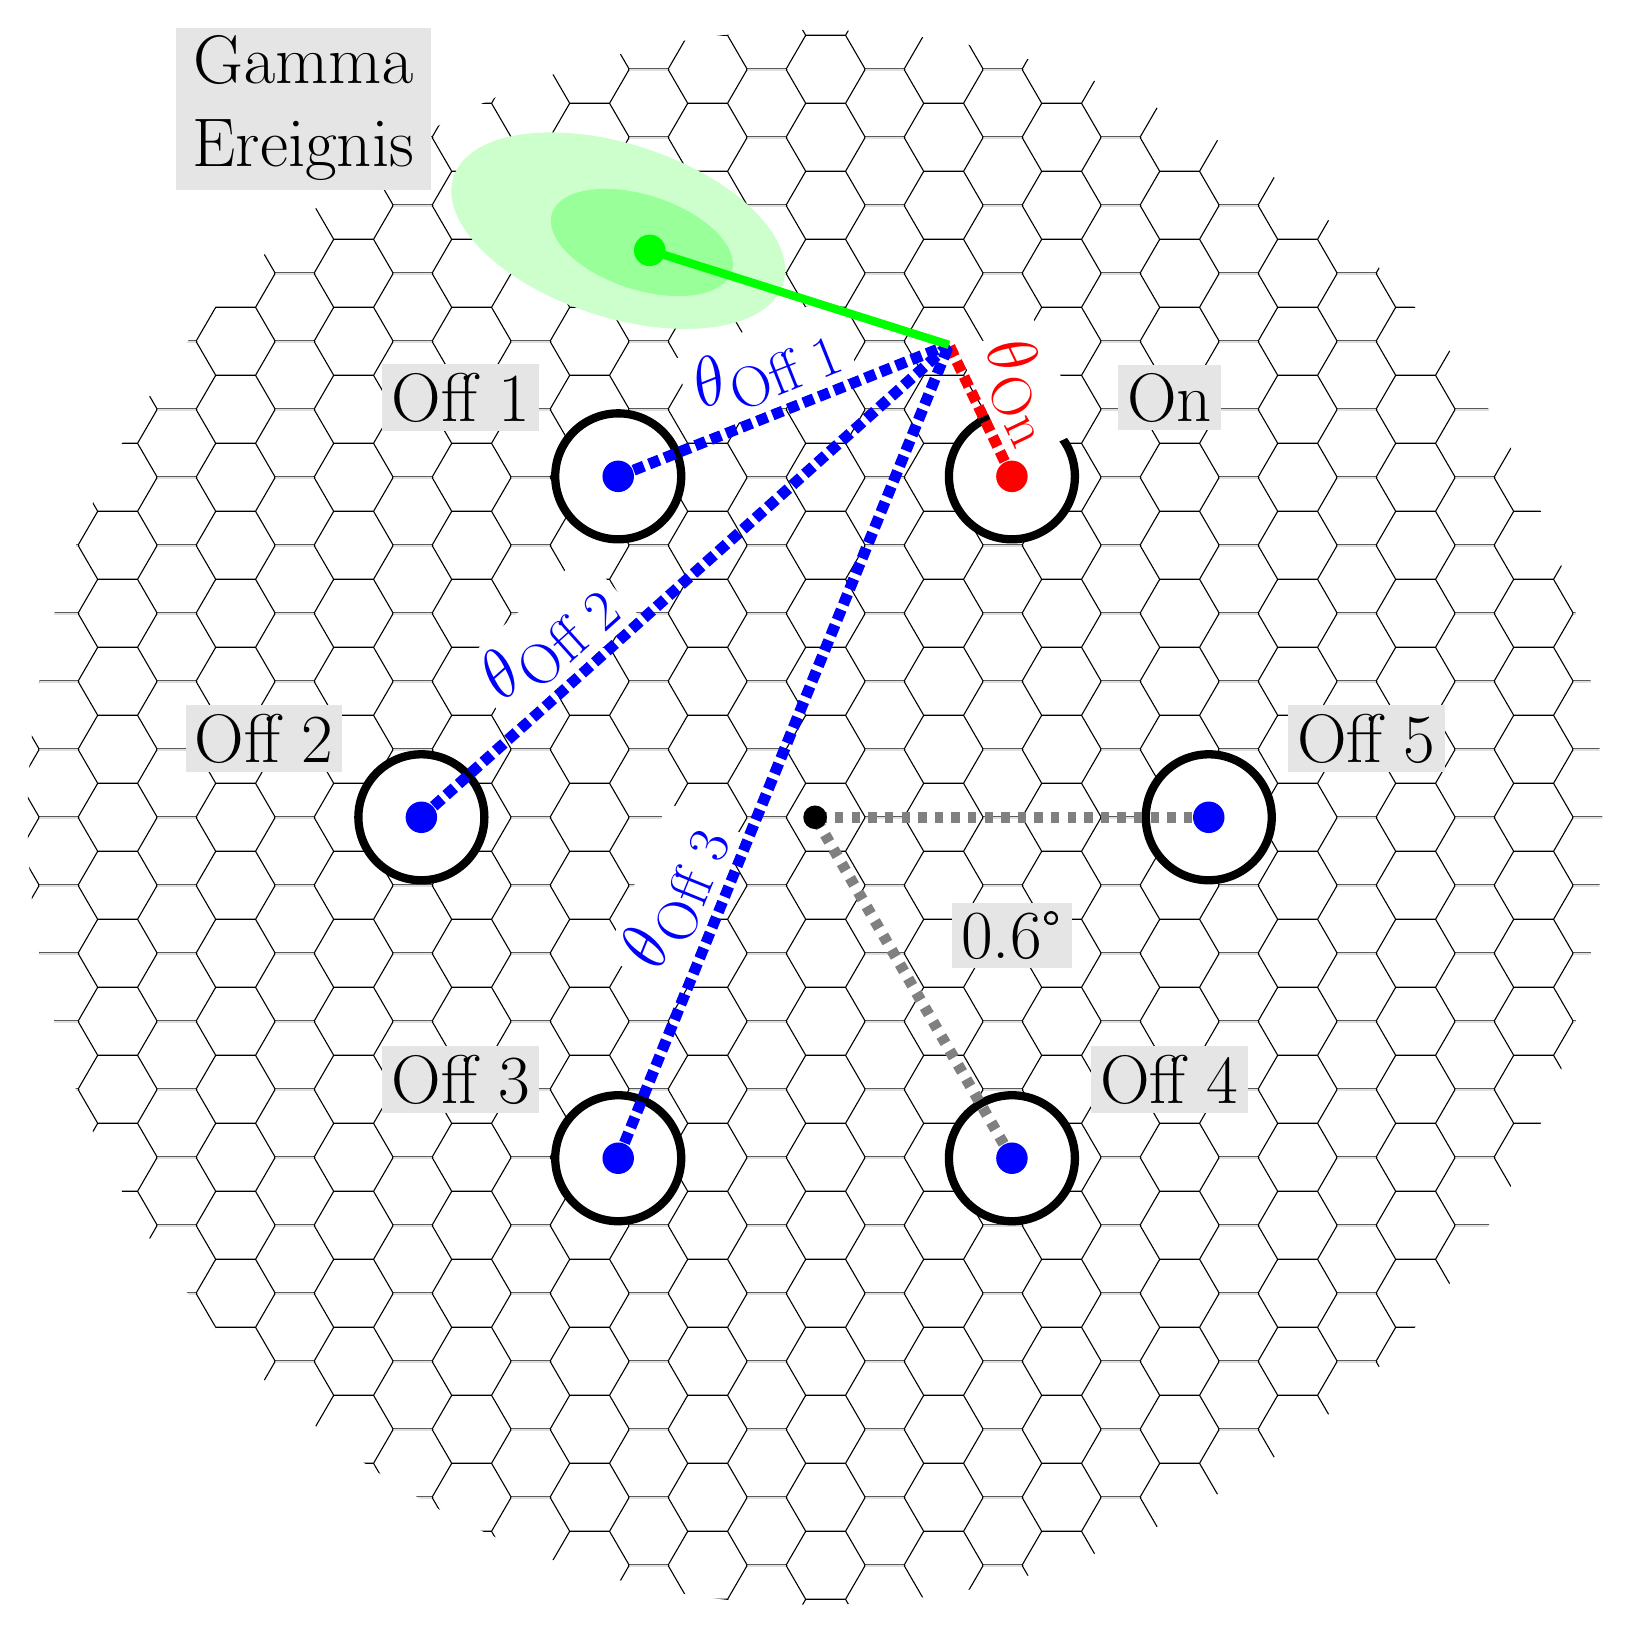
\begin{tikzpicture}
  %zeichnet hexagonales Rundes Grid
  \fill[pattern=hexagons] (0,0) circle (10cm);
 

  %Region expected source
  \draw[line width=3pt, fill=white] (5 , 0) 		circle [radius=.8];
  \draw[line width=3pt, fill=white] (2.5 , 4.33) 	circle [radius=.8];
  \draw[line width=3pt, fill=white] (-2.5, 4.33) 	circle [radius=.8];
  \draw[line width=3pt, fill=white] (-5  , 0) 		circle [radius=.8];
  \draw[line width=3pt, fill=white] (-2.5, -4.33) 	circle [radius=.8];
  \draw[line width=3pt, fill=white] (2.5 , -4.33) 	circle [radius=.8];

  % linien zur Source position
  \draw[red, lineStyle] (2.5 , 4.33) 	-- (1.7,6) node[textLine] {$\theta\textsubscript{On}$};
  \draw[blue, lineStyle] (-2.5, 4.33) 	-- (1.7,6) node[textLine] {$\theta\textsubscript{Off 1}$} ;
  \draw[blue, lineStyle] (-5  , 0) 		-- (1.7,6) node[textLine, pos=0.3] {$\theta\textsubscript{Off 2}$} ;
  \draw[blue, lineStyle] (-2.5, -4.33) 	-- (1.7,6) node[textLine, pos=0.3] {$\theta\textsubscript{Off 3}$} ;

  \draw[line2Style] (5 , 0) 			-- (0,0) ;
  \draw[line2Style] (2.5 , -4.33) 	-- (0,0) ;

  % Non Noff positions
  \fill[fill=blue]  	(5   , 0) 		circle [radius=0.2];
  \fill[fill=red] 		(2.5 , 4.33) 	circle [radius=0.2];
  \fill[fill=blue] 		(-2.5, 4.33) 	circle [radius=0.2];
  \fill[fill=blue] 		(-5  , 0) 		circle [radius=0.2];
  \fill[fill=blue] 		(-2.5, -4.33) 	circle [radius=0.2];
  \fill[fill=blue] 		(2.5 , -4.33) 	circle [radius=0.2];
  \fill[fill=black] 	(0 , 0) 		circle [radius=0.15];

  % Text Positions
  \node[textStyle] at (7,1) 			{Off 5};
  \node[textStyle] at (4.5 , 5.33) 		{On};
  \node[textStyle] at (-4.5, 5.33) 		{Off 1};
  \node[textStyle] at (-7  , 1) 		{Off 2};
  \node[textStyle] at (-4.5, -3.33) 	{Off 3};
  \node[textStyle] at (4.5 , -3.33) 	{Off 4};
  
  \node[textStyle] at (2.5 , -1.5) 		{0.6°};

  \fill[fill=green!20] (-2.5,7.45)  circle [x radius=22mm, y radius=11mm, rotate=-18];
  \fill[fill=green!40] (-2.2,7.3)	circle [x radius=12mm, y radius=6mm, rotate=-18];
  \fill[fill=green]    (-2.1,7.2) 	circle [radius=0.2];
  \draw[green, line width=3pt] (-2.1, 7.2) 	-- (1.7,6); %node[textLine, pos=0.3] {Quellposition} ;
  \node[textStyle,text width=3cm, align=center] at (-6.5,9) 		{Gamma Ereignis};


\end{tikzpicture}
\end{document}
